\documentclass[11pt,a4paper]{article}

% ===================== PACCHETTI =====================
\usepackage[utf8]{inputenc}
\usepackage[T1]{fontenc}
\usepackage[italian]{babel}
\usepackage{lmodern}
\usepackage{geometry}
\geometry{margin=2.5cm}
\usepackage{graphicx}
\usepackage{booktabs}
\usepackage{caption}
\usepackage{amsmath}
\usepackage{amssymb}
\usepackage{hyperref}
\hypersetup{
    colorlinks=true,
    linkcolor=blue,
    citecolor=blue,
    urlcolor=blue
}
\usepackage{xurl} % permette agli URL lunghi di andare a capo senza uscire dal margine
\usepackage{microtype} % migliora la giustificazione ed evita che testo/codice inline esca dal margine
\usepackage{float}
\usepackage{setspace}

% Migliora ulteriormente la giustificazione: consente di allentare la spaziatura
% come ultima risorsa invece di lasciare che il testo esca dal margine
\setlength{\emergencystretch}{3em}

\geometry{top=2.5cm, bottom=2.5cm, left=2.5cm, right=2.5cm}

\title{
    \vspace*{2cm} % Spazio sopra il titolo
    \textbf{Previsione dell'Insolvenza Creditizia: \\ Analisi e Modellazione}\\
    [1cm]
    
\includegraphics[width=0.3\textwidth]{images/logo_unibo.jpg}
    \vspace*{3cm} % Spazio titolo e autori
    }

\author{Mattia Galletti, Jacopo Malagoli, Vera Efua Van Dyke
    \vspace{1cm}
    }
    
\date{
    \vspace{0.5cm}   
    \normalsize Progetto di fine corso -- Gruppo 11 \\ 
    \normalsize Introduzione alla Data Science e al Pensiero Computazionale \\ \normalsize a.a.\ 2025/2026
    }

\begin{document}

\maketitle
\newpage 
\tableofcontents %inserimento delle lista degli argomenti
\newpage
\listoffigures % lista figure
\newpage
% ===================== ABSTRACT =====================
\begin{abstract}
\noindent
Il presente progetto sviluppa un modello predittivo per stimare il rischio di insolvenza creditizia (default) nel comparto carte di credito, a partire dal dataset fornito come materiale del progetto, relativo ad un campione di 30.000 clienti di un istituto di credito taiwanese. Dopo la fase di data cleaning e di analisi esplorativa (EDA), sono stati implementati e messi a confronto tre modelli di classificazione: Regressione Logistica, k-Nearest Neighbors (k-NN) e Random Forest. Quest'ultimo ha mostrato le prestazioni migliori (accuracy 81.1\%, F1-score 45.8\% sulla classe di default). L'efficacia predittiva di tutti i modelli risulta tuttavia fortemente condizionata dal forte sbilanciamento delle classi (77.7\% clienti regolari contro 22.3\% in default). Infine, l'analisi esplorativa, di correlazione e di feature importance ha confermato che le variabili relative ai ritardi nei pagamenti sono i predittori con il maggior potere discriminante.

\vspace{3.5em}
\noindent \textbf{Codice e notebook:} \url{https://github.com/MattiaGalletti2001/progetto-data-science-gruppo-11-credit-card-default}
\end{abstract}
\newpage
% ===================== SEZIONE 1 =====================
\section{Introduzione}

La previsione del rischio di credito è un problema centrale nel settore bancario, con implicazioni significative per la gestione del rischio finanziario \cite{altman1968}.

Negli ultimi decenni, l'avvento dei sistemi informativi e l'accumulo di ingenti moli di dati hanno spinto gli istituti di credito a transitare da metodologie di valutazione tradizionali verso sistemi avanzati di \emph{credit scoring} basati sul \emph{machine learning}, capaci di estrarre pattern non lineari dai profili comportamentali dei clienti \cite{yeh2009}.

In questo progetto affrontiamo un problema di classificazione binaria, con l'obiettivo di prevedere se un cliente andrà in default sul pagamento della carta di credito nel mese successivo. Utilizziamo il dataset fornito come materiale del progetto, originariamente raccolto e analizzato da Yeh e Lien \cite{yeh2009}, che contiene 30.000 record di un istituto di credito taiwanese e 25 variabili di natura demografica, finanziaria e legata all'andamento storico dei pagamenti precedenti.

L'obiettivo principale dello studio consiste nel confrontare l'efficacia predittiva di diverse architetture di previsione di tipo algoritmico, quali la Regressione Logistica, il \emph{k-Nearest Neighbors} (k-NN) e la Random Forest \cite{breiman2001}, valutandone criticamente la capacità di intercettare i soggetti a rischio a fronte di un marcato sbilanciamento delle classi, fenomeno intrinseco e ricorrente nei problemi di classificazione legati alle frodi e al rischio di credito \cite{fawcett2006}.

Il report è organizzato come segue: la Sezione~\ref{sec:dataset} descrive il dataset, la pulizia dei dati e l'analisi esplorativa; la Sezione~\ref{sec:metodologia} presenta la metodologia di modellazione; la Sezione~\ref{sec:risultati} riporta i risultati ottenuti, incluse le prestazioni dei modelli e l'analisi di feature importance; la Sezione~\ref{sec:discussione} discute criticamente i risultati; la Sezione~\ref{sec:conclusioni} conclude il lavoro delineando le prospettive future.

\newpage
% ===================== SEZIONE 2 =====================
\section{Dataset}
\label{sec:dataset}

\subsection{Descrizione e qualità dei dati}

Il dataset \texttt{Credit\_Card\_Default.csv} è costituito da dati di tipo numerico (\texttt{int64}). La variabile target è \texttt{default payment next month}, codificata con 0 per i clienti regolari e 1 per i clienti in stato di insolvenza. Le variabili predittive comprendono:

\begin{itemize}
    \item \textbf{Caratteristiche demografiche}: sesso (\texttt{SEX}), istruzione (\texttt{EDUCATION}), stato civile (\texttt{MARRIAGE}), età (\texttt{AGE});
    \item \textbf{Caratteristiche finanziarie}: limite di credito (\texttt{LIMIT\_BAL}), importi fatturati negli ultimi 6 mesi (\texttt{BILL\_AMT1--6}), importi pagati (\texttt{PAY\_AMT1--6});
    \item \textbf{Storico dei ritardi nei pagamenti}: \texttt{PAY\_0, PAY\_2, \dots, PAY\_6}.
\end{itemize}

L'ispezione iniziale non ha evidenziato la presenza di valori nulli. Il controllo dei range plausibili per ciascuna variabile ha invece rilevato alcune anomalie: 345 osservazioni con valori non validi in \texttt{EDUCATION} (0, 5, 6, corrispondenti a categorie non definite), 54 osservazioni con valore 0 in \texttt{MARRIAGE}, e valori negativi nelle variabili \texttt{BILL\_AMT1--BILL\_AMT6}. Questi ultimi sono stati interpretati come rettifiche contabili o crediti residui e pertanto mantenuti nel dataset, in quanto rappresentano informazioni plausibili e non errori di inserimento.

\subsection{Pulizia dei dati}

È stata eseguita una procedura sistematica di filtraggio delle anomalie riscontrate nelle variabili categoriche \texttt{EDUCATION} e \texttt{MARRIAGE}, che sono state rimosse. L'ispezione ha rivelato che i record non validi per la variabile \texttt{EDUCATION} (codificati con i valori non censiti 0, 5 e 6) e per la variabile \texttt{MARRIAGE} (codificati con il valore anomalo 0) rappresentano a tutti gli effetti informazioni non classificabili (\emph{unknown}). La loro incidenza complessiva (circa l'1.3\% del totale) ne ha permesso l'eliminazione, rispetto a tecniche di imputazione (come la sostituzione con la moda o il valore mediano), per evitare l'introduzione di bias artificiali nella distribuzione delle frequenze delle feature demografiche.

Al termine del processo di pulizia, il dataset definitivo risulta composto da 29.601 osservazioni, utilizzate per tutte le analisi successive.

\subsection{Sbilanciamento della variabile target}

La variabile target risulta fortemente sbilanciata: il 77.7\% dei clienti è regolare nei pagamenti, mentre il 22.3\% risulta in default. Questo squilibrio rappresenta la principale sfida per la fase di modellazione. In presenza di distribuzioni asimmetriche, l'adozione dell'\emph{accuracy} come metrica principale può risultare fuorviante (poiché tende a riflettere unicamente la performance sulla classe maggioritaria); per tale motivo, la letteratura scientifica \cite{fawcett2006} suggerisce l'impiego di metriche di valutazione focalizzate sulla classe minoritaria, quali \emph{precision}, \emph{recall} e \emph{F1-score}, per quantificare correttamente la reale capacità discriminante dei modelli.

Le principali statistiche descrittive del dataset ripulito sono riassunte in Tabella~\ref{tab:statistiche}.

\begin{table}[H]
\centering
\caption{Sintesi delle principali statistiche descrittive del dataset ripulito.}
\label{tab:statistiche}
\begin{tabular}{lll}
\toprule
\textbf{Categoria} & \textbf{Descrizione} & \textbf{Valore} \\
\midrule
Target & Clienti regolari (No default) & 77.7\% \\
Target & Clienti in default (Yes) & 22.3\% \\
LIMIT\_BAL & Media complessiva (min -- max) & 167.550 (10.000 -- 1.000.000) \\
LIMIT\_BAL & Media (regolari / default) & 178.300 / 130.125 \\
LIMIT\_BAL & Correlazione con default & $r = -0.154$ \\
AGE & Media complessiva & 35.46 anni \\
AGE & Media (regolari / default) & 35.39 / 35.71 anni \\
PAY\_0 & Rischio default (puntuale $\rightarrow$ 1 mese ritardo) & 12.9\% $\rightarrow$ 34.2\% \\
PAY\_0 & Rischio default (2 mesi di ritardo) & 69.6\% \\
SEX & Tasso di default (Maschi / Femmine) & 24.36\% / 20.97\% \\
\bottomrule
\end{tabular}
\end{table}

\subsection{Variabili demografiche}

Per valutare l'associazione tra le variabili categoriche (\texttt{SEX}, \texttt{EDUCATION}, \texttt{MARRIAGE}) e il default è stato applicato il test del $\chi^2$ di indipendenza \cite{poggi2025}. I risultati, riportati in Tabella~\ref{tab:chi2}, mostrano che tutte e tre le variabili presentano un'associazione statisticamente significativa con il default ($p$-value $< 0.001$ in tutti i casi).

\begin{table}[H]
\centering
\caption{Risultati del test $\chi^2$ per le variabili demografiche categoriche.}
\label{tab:chi2}
\begin{tabular}{lccc}
\toprule
\textbf{Variabile} & $\boldsymbol{\chi^2}$ & \textbf{Gradi di libertà} & \textbf{$p$-value} \\
\midrule
SEX       & 46.73  & 1 & $8.15 \times 10^{-12}$ \\
EDUCATION & 118.72 & 3 & $1.45 \times 10^{-25}$ \\
MARRIAGE  & 32.00  & 2 & $1.13 \times 10^{-7}$ \\
\bottomrule
\end{tabular}
\end{table}

Nonostante la significatività statistica, la forza di tali associazioni è debole: per \texttt{EDUCATION} il coefficiente di V di Cramer è pari a $V = 0.063$, un valore che indica un legame modesto tra istruzione e default. Per lo stato civile, il confronto tramite Odds Ratio (OR) mostra che gli odds di default sono pari a 0.310 per i clienti sposati e 0.267 per i single; l'Odds Ratio tra i due gruppi è pari a 0.860, indicando un rischio di insolvenza leggermente inferiore per i single rispetto ai coniugati. Per quanto riguarda l'età, non emergono differenze rilevanti tra le due classi (come evidenziato nella Tabella~\ref{tab:statistiche}), suggerendo che questo fattore non è un forte discriminante del comportamento di pagamento.

\subsection{Limite di credito e default}

Il limite di credito medio complessivo è pari a 167.550 (con un range compreso tra un minimo di 10.000 ed un massimo di 1.000.000). Suddividendo il campione in base allo stato di default, i clienti regolari presentano un limite medio più elevato (178.300) rispetto ai clienti in default (130.125). Questa asimmetria è confermata da un coefficiente di correlazione lineare di Pearson pari a $r = -0.154$. Tale valore mostra una relazione parzialmente negativa, indicando una minore affidabilità creditizia corrispondente a un minore credito concesso. In Figura~\ref{fig:fig1}, la mediana del limite di credito scende da 150.000 per i clienti regolari a 90.000 per quelli in default, indicando che ai clienti considerati più rischiosi vengono generalmente concessi limiti più contenuti, confermando quanto evidenziato.

\begin{figure}[H]
    \centering
    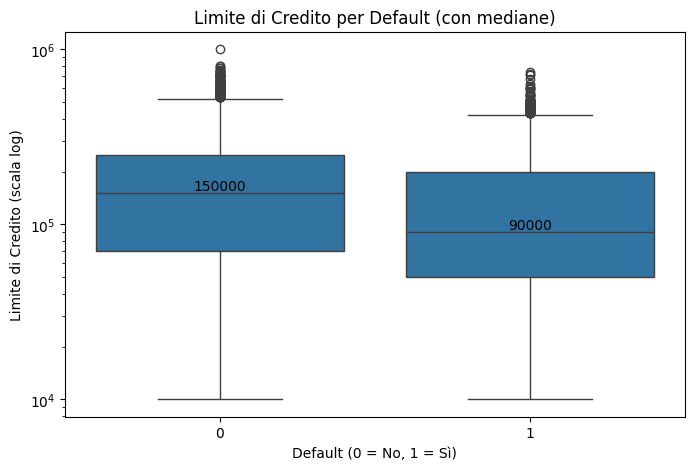
\includegraphics[width=0.55\textwidth]{images/fig1_limit_bal_boxplot.png}
    \caption{Distribuzione del limite di credito per classe di default.}
    \label{fig:fig1}
\end{figure}

\subsection{Ritardi nei pagamenti}

L'analisi del ritardo di pagamento più recente (\texttt{PAY\_0}) evidenzia una relazione fortemente non lineare con la probabilità di default (Figura~\ref{fig:fig2}). I clienti puntuali o in anticipo (\texttt{PAY\_0} $\le 0$) presentano un rischio di default compreso tra il 12.9\% e il 16.9\%. Già un mese di ritardo (\texttt{PAY\_0} $= 1$) porta il rischio al 34.2\%, mentre con due mesi di ritardo la probabilità sale al 69.6\%. Questa soglia critica suggerisce che interventi precoci, applicati già al primo mese di ritardo, potrebbero essere particolarmente efficaci nel contenere il rischio di insolvenza.

\begin{figure}[H]
    \centering
    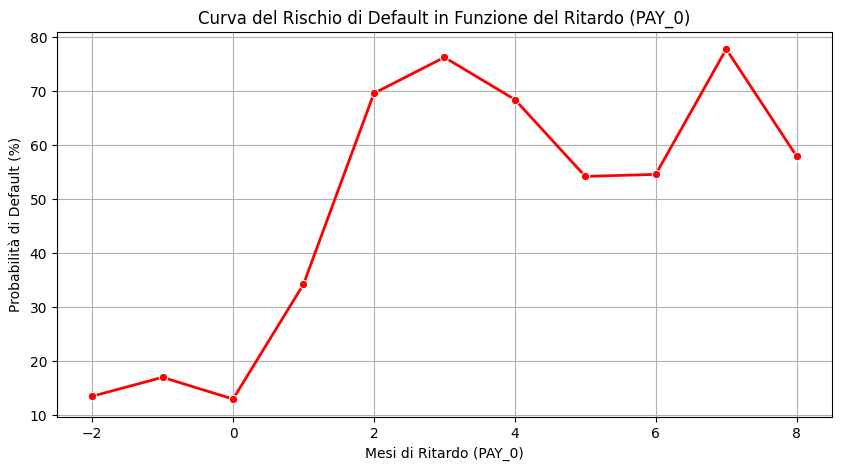
\includegraphics[width=0.85\textwidth]{images/fig2_pay0_default_prob.png}
    \caption{Probabilità di default in funzione del ritardo di pagamento più recente (\texttt{PAY\_0}).}
    \label{fig:fig2}
\end{figure}

\subsection{Correlazioni tra le variabili}

L'analisi basata sul coefficiente di correlazione lineare di Pearson (Figura~\ref{fig:fig3}) fornisce una visione d'insieme delle relazioni lineari tra le variabili del dataset e il comportamento di insolvenza.

Le variabili che presentano la più marcata associazione lineare positiva con la variabile target sono quelle relative allo storico recente dei ritardi nei pagamenti: nello specifico, \texttt{PAY\_0} ($r = 0.32$), \texttt{PAY\_2} ($r = 0.26$) e \texttt{PAY\_3} ($r = 0.24$). Al contrario, come precedentemente evidenziato, il limite di credito concesso (\texttt{LIMIT\_BAL}) mostra una correlazione negativa pari a $r = -0.154$, suggerendo che un minor affidamento si associa a un incremento del rischio di default.

Sotto il profilo metodologico, l'ispezione della matrice rivela due importanti fenomeni di collinearità:

\begin{itemize}
    \item \textbf{Altissima correlazione interna ai saldi di spesa}: si registrano valori estremamente elevati tra gli importi fatturati nei diversi mesi (\texttt{BILL\_AMT1}--\texttt{BILL\_AMT6}), con coefficienti che superano sistematicamente la soglia di $r > 0.90$. Questa forte intercorrelazione riflette la persistenza del debito residuo nel tempo. In letteratura, la presenza di una simile multicollinearità rappresenta un limite noto per i modelli lineari tradizionali (come la Regressione Logistica), in quanto può destabilizzare la stima dei coefficienti, mentre risulta più facilmente gestibile da modelli non parametrici o basati su alberi decisionali \cite{yeh2009,breiman2001}.
    \item \textbf{Continuità nei comportamenti di ritardo}: si osservano correlazioni moderate-alte tra i diversi indicatori di ritardo sequenziali (\texttt{PAY\_0}--\texttt{PAY\_6}, con picchi fino a $r = 0.67$), indice di una forte inerzia comportamentale nei pagamenti da parte del cliente.
\end{itemize}

Al contrario, tutte le caratteristiche demografiche (\texttt{SEX}, \texttt{EDUCATION}, \texttt{MARRIAGE}, \texttt{AGE}) mostrano un'associazione lineare pressoché nulla con la variabile target ($|r| < 0.05$). Tale evidenza suggerisce, ai fini della previsione del rischio di credito, che le informazioni di tipo strettamente comportamentale e finanziario abbiano un potere informativo nettamente superiore rispetto alle variabili anagrafiche del titolare della carta \cite{yeh2009}.

\begin{figure}[H]
    \centering
    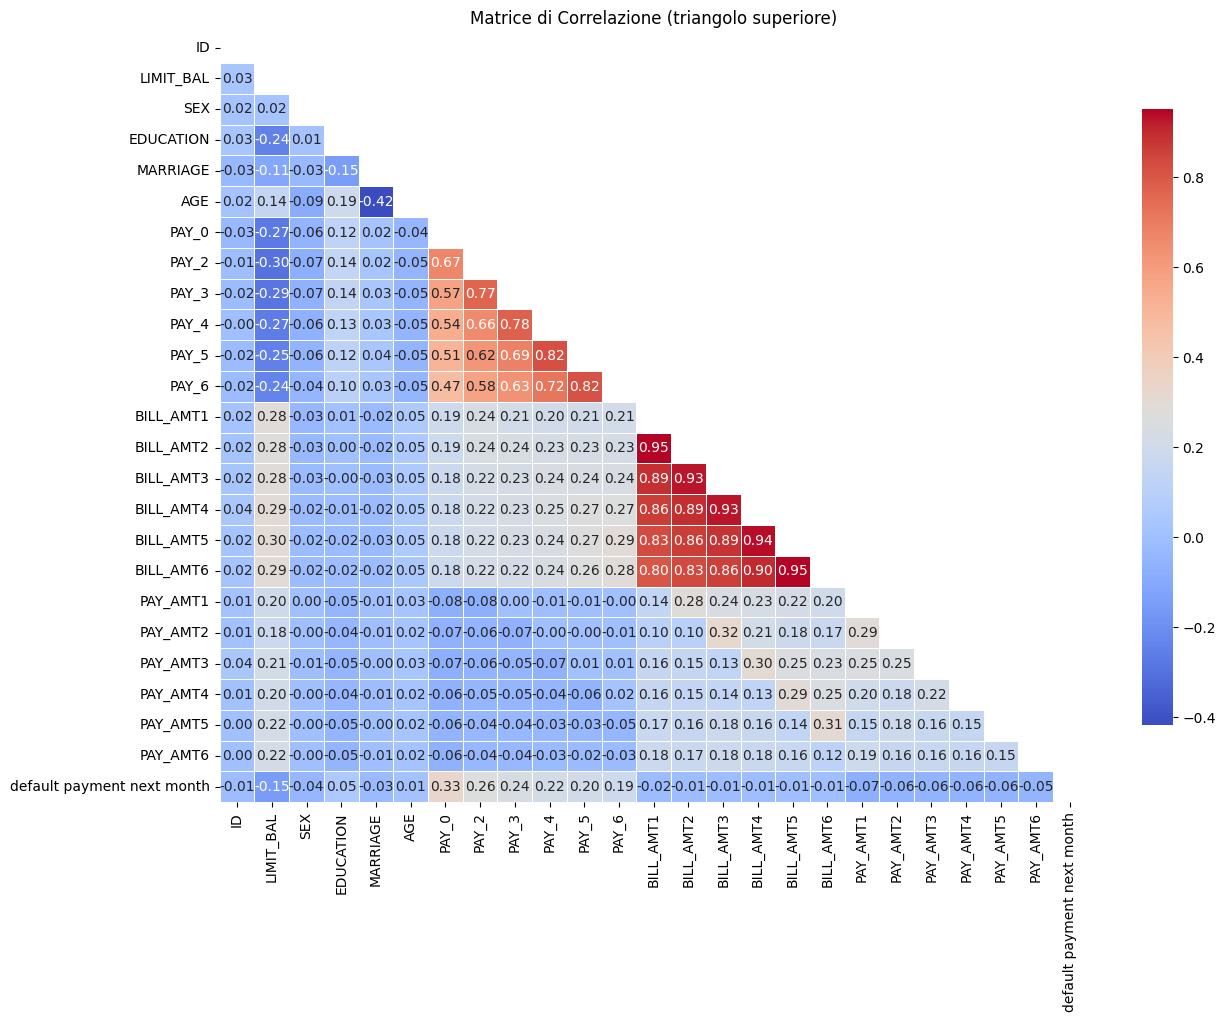
\includegraphics[width=0.85\textwidth]{images/fig3_correlation_matrix.png}
    \caption{Matrice di correlazione di Pearson tra le variabili del dataset.}
    \label{fig:fig3}
\end{figure}
\newpage
% ===================== SEZIONE 3 =====================
\section{Metodologia}
\label{sec:metodologia}

Il dataset ripulito è stato suddiviso in un insieme di training (80\%, 23.680 osservazioni) e uno di verifica (test set del 20\%, pari a 5.921 osservazioni), con stratificazione rispetto alla variabile target per preservare la proporzione tra le due classi in entrambi gli insiemi. Al fine di preservare l'esatta proporzione tra clienti regolari e in insolvenza in entrambe le partizioni ed evitare distorsioni nella valutazione, la separazione è stata condotta tramite campionamento stratificato rispetto alla variabile target, una tecnica utilizzata in presenza di distribuzioni fortemente sbilanciate \cite{fawcett2006}.

Le variabili numeriche sono state inoltre standardizzate tramite \texttt{StandardScaler}, passaggio necessario per la Regressione Logistica e per il k-NN, algoritmi sensibili alla scala delle feature. La standardizzazione trasforma ogni feature $x$ in modo che abbia media $\approx 0$ e deviazione standard $\approx 1$:
\begin{equation}
    z = \frac{x - \mu}{\sigma},
    \label{eq:standardization}
\end{equation}
dove $\mu$ e $\sigma$ sono rispettivamente la media e la deviazione standard calcolate \emph{esclusivamente sul training set}, per evitare fenomeni di \emph{data leakage} verso il test set. La Random Forest, non basandosi su misure di distanza, è stata invece addestrata sui dati non standardizzati \cite{poggi2025}.

\begin{description}
    \item[Regressione Logistica:] modella la probabilità di default a partire da una combinazione lineare delle variabili esplicative
    \begin{equation}
        z = \beta_0 + \sum_{i=1}^{n} \beta_i x_i,
        \label{eq:linear-combination}
    \end{equation}
    trasformata poi tramite la funzione sigmoide, che schiaccia l'output nell'intervallo $[0,1]$:
    \begin{equation}
        \sigma(z) = \frac{1}{1 + e^{-z}} = P(y=1 \mid \mathbf{x}).
        \label{eq:sigmoid}
    \end{equation}
    Qui $\beta_0$ è l'intercetta, $\beta_i$ sono i coefficienti stimati per ciascuna variabile esplicativa $x_i$, e $P(y=1 \mid \mathbf{x})$ rappresenta la probabilità stimata di default dato il vettore di feature $\mathbf{x}$. Una soglia decisionale (tipicamente 0.5) converte poi questa probabilità in una classe predetta. È un modello semplice e interpretabile, utilizzato come baseline per il confronto con i modelli successivi \cite{poggi2025}.
    \item[k-Nearest Neighbors (k-NN):] classifica una nuova osservazione in base alla classe maggioritaria tra i $k$ vicini più prossimi nello spazio delle feature, secondo la distanza euclidea. È stato scelto $k = 5$. Trattandosi di un modello basato sulla similarità locale, la standardizzazione delle variabili è cruciale per evitare che feature con range di valori più ampi (ad es. \texttt{LIMIT\_BAL}, \texttt{BILL\_AMT}) dominino il calcolo delle distanze \cite{poggi2025}.
    \item[Random Forest:] modello ensemble basato sulla combinazione di 100 alberi decisionali (\texttt{n\_estimators\allowbreak=100}), in cui la determinazione della classe finale avviene per voto di maggioranza \cite{breiman2001}. Così come indicato dalla formulazione teorica di Breiman \cite{breiman2001}, l'algoritmo introduce una doppia componente di casualità: il \emph{bagging} (campionamento con reinserimento per l'addestramento dei singoli alberi) e la selezione casuale di un sottoinsieme di feature ad ogni nodo di splitting (\emph{feature bagging}). Questa struttura riduce la correlazione tra gli alberi, minimizzando la varianza del modello senza inficiare la stabilità, e consente di mappare relazioni non lineari e interazioni complesse tra i dati finanziari senza alcuna necessità di standardizzazione preventiva dei dati \cite{poggi2025}.
\end{description}

\newpage
% ===================== SEZIONE 4 =====================
\section{Risultati}
\label{sec:risultati}

\subsection{Confronto dei modelli}

Di seguito vengono riportati i risultati derivanti dal confronto dei modelli.\\
Le prestazioni dei tre modelli sulla classe di default (classe minoritaria, 1) sono riportate in Tabella~\ref{tab:confronto}.

\begin{table}[H]
\centering
\caption{Confronto delle prestazioni dei modelli sulla classe di default.}
\label{tab:confronto}
\begin{tabular}{lcccc}
\toprule
\textbf{Modello} & \textbf{Accuracy} & \textbf{Precision} & \textbf{Recall} & \textbf{F1-score} \\
\midrule
Regressione Logistica & 0.810 & 0.720 & 0.241 & 0.362 \\
k-NN ($k=5$)          & 0.784 & 0.525 & 0.338 & 0.411 \\
Random Forest         & 0.811 & 0.636 & 0.358 & 0.458 \\
\bottomrule
\end{tabular}
\end{table}
 Come evidenziato nella tabella la Random Forest è il modello più performante, con la migliore accuracy (0.8110), il miglior F1‑score (0.4581) e il recall più alto, mostrando la maggiore capacità di individuare i clienti insolventi.
La Logistic Regression ha un’accuracy simile ma privilegia la precisione (0.7201), sacrificando il recall e perdendo molti casi di default.
Il k‑NN offre risultati intermedi: recall superiore alla Logistic Regression ma accuracy e F1‑score inferiori alla Random Forest.

Le matrici di confusione mostrano che tutti i modelli faticano a identificare correttamente i clienti in default, con un numero elevato di falsi negativi (clienti classificati come regolari ma effettivamente in default), coerentemente con lo sbilanciamento del dataset.

\begin{figure}[H]
    \centering

    \begin{minipage}{0.32\textwidth}%adattamento delle figure
        \centering
        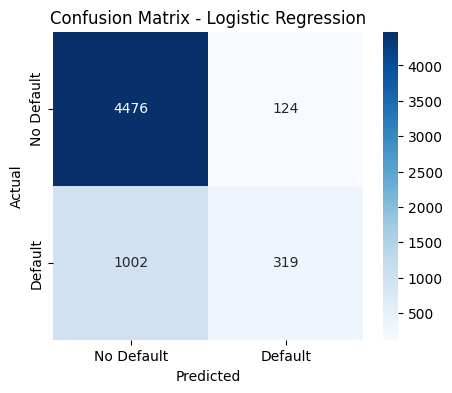
\includegraphics[width=\textwidth]{images/fig_confusion_logistic.png}
        \caption{Logistic Regression}
        \label{fig:cm-logistic}
    \end{minipage}
    \hfill
    \begin{minipage}{0.32\textwidth}
        \centering
        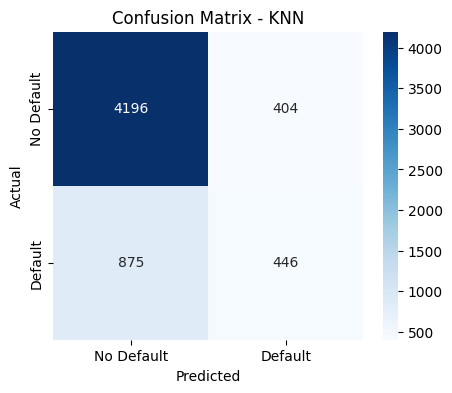
\includegraphics[width=\textwidth]{images/fig_confusion_knn.png}
        \caption{k-NN}
        \label{fig:cm-knn}
    \end{minipage}
    \hfill
    \begin{minipage}{0.32\textwidth}
        \centering
        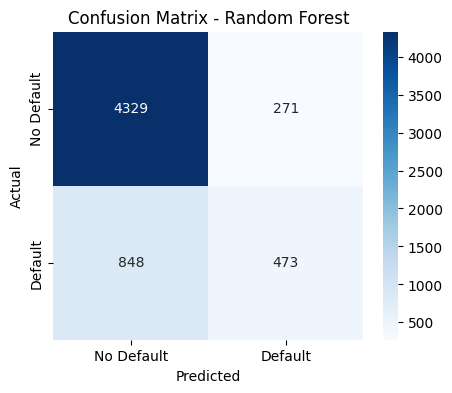
\includegraphics[width=\textwidth]{images/fig_confusion_rf.png}
        \caption{Random Forest}
        \label{fig:cm-rf}
    \end{minipage}

\end{figure}


\newpage
\subsection{Importanza delle variabili (Random Forest)}

Per interpretare il funzionamento del modello migliore, è stata calcolata l'importanza relativa delle variabili nella Random Forest (Figura~\ref{fig:fig4}). Questo processo di interpretazione si basa sul principio introdotto da Breiman (2001), secondo cui l'impatto di ciascun descrittore viene stimato misurando la degradazione delle prestazioni del modello quando i valori della variabile nei campioni \emph{Out-of-Bag} (OOB) vengono permutati casualmente \cite{breiman2001}.

Lo storico dei ritardi nei pagamenti (\texttt{PAY\_0}, \texttt{PAY\_2}, \texttt{PAY\_3}, \dots) risulta il principale fattore predittivo del default, seguito da alcune variabili economiche come il limite di credito e gli importi delle fatture. Questo risultato è coerente con quanto emerso nell'analisi esplorativa (Sezione~\ref{sec:dataset}), confermando che lo storico di pagamento -- e non le caratteristiche anagrafiche -- guida la capacità predittiva del modello.

\begin{figure}[H]
    \centering
    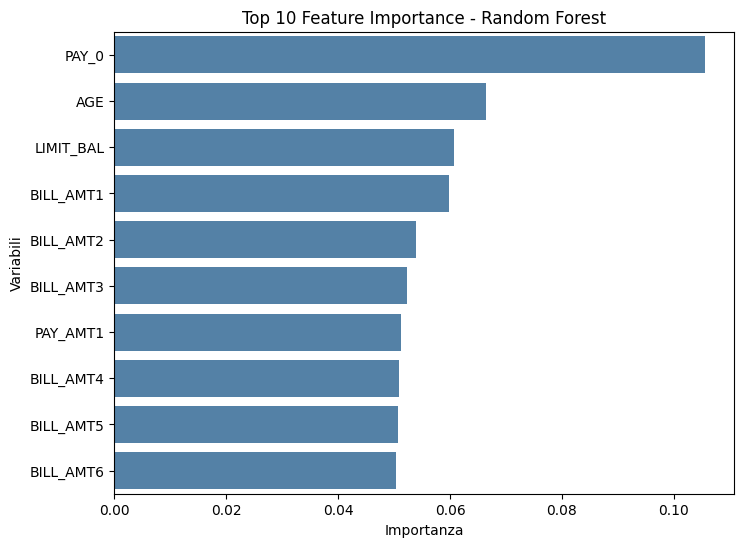
\includegraphics[width=0.55\textwidth]{images/fig4_feature_importance.png}
    \caption{Importanza delle variabili nella Random Forest -- prime 10 variabili.}
    \label{fig:fig4}
\end{figure}

\newpage
% ===================== SEZIONE 5 =====================
\section{Discussione}
\label{sec:discussione}

I risultati mostrano un chiaro trade-off tra precision e recall. La Regressione Logistica ottiene la precision più alta (72.0\%) ma un recall molto basso (24.1\%): identifica correttamente solo un cliente su quattro tra quelli che effettivamente andranno in default, rendendola poco utile in un contesto operativo dove il costo di un mancato riconoscimento è elevato. Il k-NN migliora il recall (33.8\%) a scapito della precision (52.5\%): l'approccio basato sulla similarità locale introduce un numero maggiore di falsi positivi.

La Random Forest offre il miglior bilanciamento tra le due metriche (precision 63.6\%, recall 35.8\%, F1-score 45.8\%). Nella scelta del modello più adatto è opportuno andare oltre l'accuracy complessiva: in un contesto finanziario è generalmente preferibile identificare il maggior numero possibile di clienti a rischio, anche a costo di qualche falso positivo in più, per cui recall e F1-score risultano più rappresentativi dell'accuracy su un dataset sbilanciato -- ed entrambi premiano la Random Forest. Questa lettura è rafforzata dall'analisi di feature importance (Sezione~\ref{sec:risultati}), che individua negli stessi ritardi di pagamento recenti già emersi in EDA i predittori più rilevanti per il modello, confermando la robustezza del segnale individuato.

Un aspetto rilevante emerso dall'analisi esplorativa è la scarsa rilevanza delle variabili demografiche: nonostante il test del $\chi^2$ ne confermi la significatività statistica (Tabella~\ref{tab:chi2}), la forza dell'associazione (misurata tramite V di Cramer) resta debole, e tali variabili non compaiono tra le più importanti nella Random Forest. Ciò suggerisce che il comportamento di pagamento passato sia un indicatore molto più forte delle caratteristiche anagrafiche del cliente, e che un modello semplificato -- privo di queste variabili -- potrebbe mantenere prestazioni simili migliorando al contempo l'interpretabilità.

Il forte sbilanciamento delle classi resta la principale limitazione dello studio: tutti i modelli tendono a privilegiare la classe maggioritaria (clienti regolari), ottenendo un'accuracy elevata ma un recall contenuto sulla classe di default. Questo comportamento è tipico degli algoritmi standard quando non vengono applicate tecniche specifiche di riequilibrio delle classi (ad es. oversampling, undersampling, SMOTE, o pesi di classe).

\newpage
% ===================== SEZIONE 6 =====================
\section{Conclusioni}
\label{sec:conclusioni}

La Random Forest si conferma il modello più efficace tra quelli testati per la previsione del default sulle carte di credito, grazie al miglior bilanciamento tra precisione e recall e al valore più alto di F1-score. Il recall complessivo rimane tuttavia contenuto (35.8\%), evidenziando la necessità di affrontare lo sbilanciamento del dataset in lavori futuri, ad esempio tramite tecniche di ricampionamento o l'uso di pesi di classe.

L'analisi ha inoltre mostrato che le variabili demografiche hanno un impatto limitato sulla previsione del default, sia in termini di associazione statistica sia di importanza nel modello ad alberi, e potrebbero essere escluse per semplificare il modello senza significative perdite prestazionali, a favore di un maggiore peso delle variabili relative allo storico dei pagamenti. Questo approccio di semplificazione è supportato dalla teoria dei modelli di ensemble, in cui l'esclusione di feature deboli o scarsamente correlate al target riduce il rumore di fondo senza intaccare la convergenza quasi certa dell'errore di generalizzazione propria dell'algoritmo \cite{breiman2001}.

I risultati ottenuti sono coerenti con le evidenze raccolte lungo l'intero processo di analisi -- dall'esplorazione dei dati fino all'interpretazione del modello finale -- e forniscono una solida base per ulteriori sviluppi nell'ambito del credit scoring, in particolare per approfondimenti sulle tecniche di gestione dei dataset sbilanciati.

\newpage
% ===================== BIBLIOGRAFIA =====================

\bibliographystyle{plain}
\bibliography{bibliografia}

\end{document}